\chapter{State-of-the-art} \label{chap:State_of_the_art}

In the present chapter, a review of the current technology related to the topic of this work will be reviewed. Firstly, a review of the different morphing wing technologies will be introduced. Secondly, a particular focus on the state-of-the-art of technology exploit in the current project will be presented.

\section{Morphing aircraft} \label{sec:Morphing_state}

  The interest in morphing of the aerodynamic surfaces has accompany aerospace history since the beginning. Since the first heavier-than-air flight in 1903, when the Wright Brothers designed and build the first controlled, sustained flight of a powered heavier-than-air aircraft. Their concept of aircraft did not provide importance to built-in stability but absolute control of the aircraft by the pilot. For this reason, they deliberatively designed their first aircraft with anhedral wing that make it be dynamically unstable to perturbations in sideslip but more maneuverable in the lateral direction. In order to achieve roll control, they decided to incorporate a mechanism that would allow the wings to twist by pulling from cables, as it can be seen in Figure \ref{fig:Wright}. This was the first ever use of morphing of an aerodynamic surface for aircraft control. Since them, the necessity of enhanced performance and higher airspeed brought the requirement of stiffer wing structures to avoid aeroelastic instabilities. This caused the invention o

  \begin{figure}[!htpb]
    \centering
    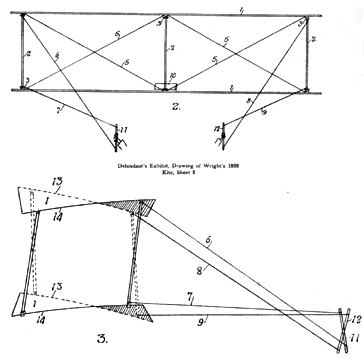
\includegraphics[width=0.8 \textwidth]{state-of-the-art/WrightBrothers1899Kite}
    \caption[Wright Brothers 1899 kite]{Wright 1899 kite: front and side views, with control sticks. Wing-warping is shown in lower view. \cite{Wright}}\label{fig:Wright}
  \end{figure}

  %Why to used them?
  On conventional aircraft, the need to modify the airflow around the airfoil at different flight conditions is achieve through discrete hinged mechanics such as flaps and ailerons. This mechanism perform well in a limited range around the design point while the outside this range, they have a negative influence in the aerodynamics. The necessary discontinuities in the surface bring forward the boundary layer transition from laminar to turbulent regime. Being able to modify the airflow without discontinuities on the airfoil skin would come along with notable reduction in fuel consumption.

  %Why now?
  New interest has raised in the recent years in aircraft morphing, mainly due to the appearance of new smart materials that allow more efficient mechanical design that do not necessarily incur weight increase \cite{Lloyd2007}. Another reason that is pushing forward new aircraft morphing technologies is that missions today are in need of higher aircraft versatility to decrease operational costs in the commercial aviation field and aim smaller and more distributed targets in the military field. For example, Airbus has recently patented a design of a downwardly foldable wing tip device applicable for a large passenger aircraft \cite{Boye2015}.

  %Different morphing projects - \cite{Barbarino}
  A general classification of different wing morphing concepts can be seen in Figure \ref{fig:morphingTypes}: planform modification through variation of sweep angle, span or chord; out-of-plane alteration involving twist, dihedral angle and spanwise bending, and airfoil adjustment achieved by modifications of the airfoil chamber and/or thickness. Under this classification, the morphing technology that is the focus of this project is located under the out-of-plane branch and twist modification.
   

  \begin{figure}[!htpb]
    \centering
    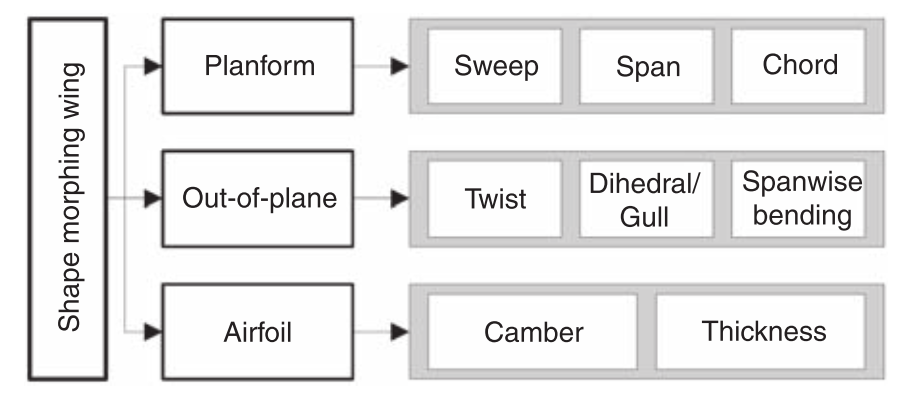
\includegraphics[width=0.8 \textwidth]{state-of-the-art/morphingTypes}
    \caption[Shape morphing wing classification]{Shape morphing wing classification. \cite{Barbarino2011}}\label{fig:morphingTypes}
  \end{figure}

  %Fundamental idea
  Morphing designs may also benefit from geo-metrically flexible structures if the aeroelastic energy from the airstream can be used to activate the shape changing and tabs can maintain the shape using aero-elastic control.

  %NASA morphing proyect

\section{Wing twist morphing} \label{sec:twist_state}

  In the present section, an analysis of different concepts used to achieve .

  The concept of modifying the wing twist to modify the airfoil exploits the 
\clearpage
\section{Compliant chiral structure} \label{sec:chiral_state}
  % \citeauthor{Lakes1991}
  % \citeauthor{Bornengo2005}
  % \citeauthor{Prall1997}

  As mentioned before, it is the interest of this work to exploit the capabilities of materials with negative Poisson's ratio. Such materials expand laterally when stretched and contract laterally when compressed. In \cite{Lakes1991}, R. Lakes proposed that negative Poisson's ratios can result from a hexagonal microstructure of rotable nodes and bendable ligaments such as the one shown in Figure \ref{fig:chiral}. Such structures are known as non-centrosymmetric, hemitropic, or chiral; they are distinguishable from their mirror image; that is, they cannot be superposed onto them and they are not isotropic.

  \begin{figure}[!htpb]
    \centering
    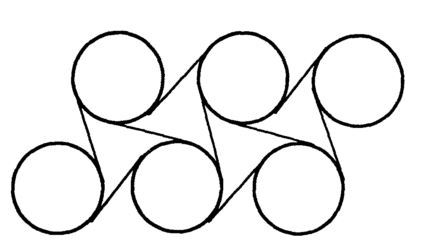
\includegraphics[width=0.8 \textwidth]{state-of-the-art/chiral}
    \caption[Chiral structure of rotable nodes and bendable ligaments]{Chiral (noncentrosymmetric) hexagonal microstructure of rotable nodes and bendable ligaments. Poisson's ratio is negative. \cite{Lakes1991}}\label{fig:chiral}
  \end{figure}

  In \cite{Prall1997}, experimental results showed that the a honeycomb chiral structure exhibited a Poisson's ratio of -1 for deformations in-plane. Indeed, this behavior was maintained over a significant range of strain, as shown in Figure \ref{fig:experimentalPoisson}, and therefore verifying that Poisson's ratio is independent upon the strain, in agreement with theory. 

  \begin{figure}[!htpb]
    \centering
    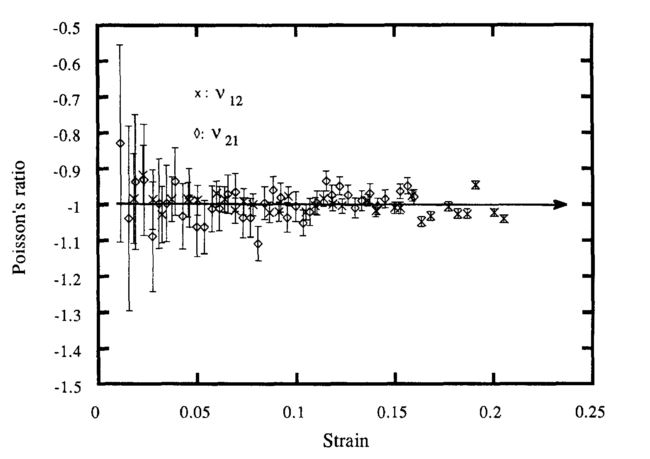
\includegraphics[width=0.8 \textwidth]{state-of-the-art/experimentalPoisson}
    \caption[Experimental Poisson's ratio $v$ as a function of axial compressive strain on a chiral honeycomb]{Experimental Poisson's ratio $\nu$ as a function of axial compressive strain on a chiral honeycomb. The error bars represent inaccuracies due to the measurement resolution. \cite{Prall1997}}\label{fig:experimentalPoisson}
  \end{figure}

  In \cite{Bettini2010} the properties of a chiral honeycomb are investigated, a manufacturing process using composite materials is proposed and the increase in the performance of using such materials is shown. Also, the experiments carried out allowed to characterize the possible failure modes of this structures and the nonlinear response when large displacements occur.

  %Buckling - Reference to work done by Gilles
  The negative Poisson’s ratio behavior leads to unique deformation patterns, and corresponds to a very high in-plane shear modulus $G$, as shown in Equation \ref{eq:shearModulus} for values of $\vu \to -1$. The high shear modulus causes the opposition of the structure to the distortion of unit cells.

  \begin{eqution}\label{eq:shearModulus}
    G = \frac{E}{2 (1 - \nu)}
  \end{eqution}

\clearpage
\section{Chiral wing rib} \label{sec:wingRibChiral_state}

  Different approaches has been followed to exploit the particular characteristics of chiral structures on aerodynamic elements such as airfoils. In \cite{Bornengo2005} a truss-core configuration such as the one shown on the upper sketch of Figure \ref{fig:truss-core-airfoil} with chiral topology was utilized to design an airfoil for automotive competitions. The concept exploit the elastic deformation of the chiral lattice to modify the airfoil mean chamber line and thus modifying the pressure distribution as required for the current desired performance of the car. In \cite{Spadoni2007a}, a similar configuration was investigated by weakly coupled structural and CFD models, and the local and global deformations were characterized by consideration of the macroscopic chiral configuration. A prototype of the proposed design such as the one shown in Figure \ref{fig:truss-core-prototype} was manufactured and tested in \cite{Spadoni2007b}. Results showed a remarkable tailoring of the chamber morphing performance by means of a limited number of parameters which define the core geometry. The dynamic properties of such chiral truss-core assemblies were investigated in \cite{Spadoni2006}.

  \begin{figure}[!htpb]
    \centering
    \includegraphics[width=0.8 \textwidth]{state-of-the-art/truss-core-airfoil}
    \caption[Investigated configurations for the truss-core of chiral topology]{Investigated configurations for the truss-core of chiral topology. \cite{Spadoni2007a}}\label{fig:truss-core-airfoil}
  \end{figure}

  \begin{figure}[!htpb]
    \centering
    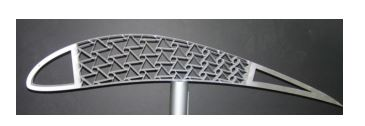
\includegraphics[width=0.8 \textwidth]{state-of-the-art/truss-core-prototype}
    \caption[Manufactured prototype of a truss-core airfoil with chiral topology]{Manufactured prototype of a truss-core airfoil with chiral topology. They were manufacture in aluminum, using water-jet cutting techniques. \cite{Spadoni2007b}}\label{fig:truss-core-prototype}
  \end{figure}

  In the recent years, A. Airoldi developed the ``chiral sail'' concept in \cite{Airoldi2012} which exploits the chiral topology of a embed chiral network is embed into the airfoil rib. The pressure different between the upper and lower parts of the airfoil promotes the chamber variation as shown in Figure XX and amplifying the lift when the angle of attack increases. This concept was implemented and validated in \cite{Airoldi2015a} in a demonstrator. The experimental side of this work showed the difficulties of manufacturing such complex structures.

  \begin{figure}[!htpb]
    \centering
    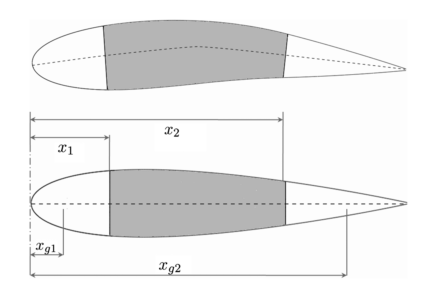
\includegraphics[width=0.8 \textwidth]{state-of-the-art/chiral-sail}
    \caption[Chiral sail concept]{Chiral sail concept. The rib of the airfoil is constituted of a network of chiral unit cells \cite{Airoldi2012}}\label{fig:truss-core-prototype}
  \end{figure}  

  \clearpage
  \section{Bending-Twist shape adaptation by compliant structural designs}
  %Mention-> Falk's work, compare with the actual design proposal (chiral structure): Compliant Chiral Spar Design, 
  
  % by designing structural components in which instability occurs in a deliberate way. For that purpose, a structural tailoring procedure providing a particular material anisotropy by varying fibre orientation and thickness of the component is introduced.
  % carbon fibre reinforced plastic (CFRP)

  The concept is presented in \cite{Raither2013a} and exploit in \cite{Raither2013}, using the consisting in using the temperature dependence of the elastic modulus of polymers in proximity of their glass transition which was presented in \cite{Raither2012}. 

  \clearpage
  \section{Current project}

  For the investigation presented in this work, the capabilities of the presented chiral structures are exploit in a different manner. For most of the works presented in this chapter, the object to be 

  Those, papers that investigate the use variable stiffness structures on the wing-box used different variable-stiffness technologies such as temperature-variable polymers or providing particular material anisotropy boundary by properties on the composite material .

  % Such solutions obtain the required performances for a pre-defined shape variation and are optimized for a
  % ligaments. Such solutions obtain the required performances for a pre-defined shape variation and are optimized for a
  % given actuation lay-out, whereas the adoption of a structural
  % concept such as the chiral honeycomb offers the possibility
  % of multiple combinations of actuation forces, so to
  % potentially provide a variety of morphing functionalities
  % with a single structural design.

  a novel application of the chiral elements is exploit. In particular, its buckling capabilities are used in a spar design 

